$  $\pagebreak
\subsection{Software Design}

\subsubsection{Purpose}

The purpose of the On-Board Software consisted of:
\begin{itemize}
    \item Controlling the selecting and tracking of targets to observe.
    \item Ensuring that the camera is not oriented towards the sun.
    \item Reading data from sensors and controlling actuators when needed.
    \item Processing and storing images taken by camera.
    \item Logging housekeeping data.
    \item When possible, sending images and housekeeping data to ground station.
\end{itemize}

The software was designed such that it can control the experiment autonomously throughout the whole experiment process but also enable control from ground through telecommands.

\subsubsection{Design}
\label{sec:4.8.2}

\paragraph{a)} Process Overview

\begin{figure}[H]
    \centering
    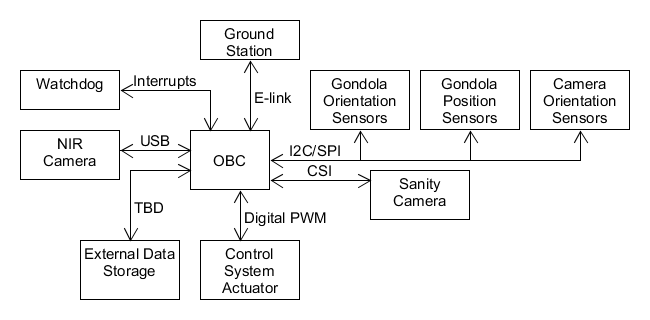
\includegraphics[width=.9\textwidth]{4-experiment-design/img/software/process-overview.png}
    \caption{Relations between On-Board Computer and connected components.}
    \label{fig:software-process-overview}
\end{figure}

All external components connected to the On-Board Computer and their interface are displayed in figure \ref{fig:software-process-overview}. The guiding camera provided an overall view in the direction the telescope was pointing and was also used as a star tracker to determine the gondola attitude.

\paragraph{b)} General and safety related concepts

To ensure that the software would not be erroneous rigorous testing was planned to be done during development and after completion. However, due to lack of time and mediocre planning, parts of the software were not tested as thoroughly as desired. A watchdog timer was used to avoid failure due to software freezing. This timer would reset the On-Board Computer if it were not itself reset by the software within a certain period.

\paragraph{c)} Interfaces

All communications over the E-link was done using TCP to ensure that packet loss wouldn't corrupt data.

\begin{table}[H]
	\centering
	\begin{tabular}{l|l}
		\textbf{Component}
		& \textbf{Interface} \\ \hline
		Ground Station
		& E-link             \\
		NIR Camera
		& USB                \\
		Guiding Camera
		& USB                \\
		Gondola GPS
		& SPI                \\
		Telescope Gyroscope
		& I2C                \\
		Telescope Encoders
		& I2C                \\
		Controller Actuators
		& I2C                \\
		Thermal Sensors
		& I2C				 \\
		Heaters \& Coolers
		& I2C
	\end{tabular}
	\caption{Table showing the interface that each external component was connected with. This is also visually represented in figure \ref{fig:software-process-overview}.}
	\label{tab:software-interfaces}
\end{table}


The data rate requested was 300\,kbit/s. This was calculated with the assumption that guiding images would be transmitted to ground regularly. Instead, the choice was made to only transmit housekeeping data causing the required data rate to drop drastically.

The telecommands were very small compared to the telemetry. In the worst case scenario the command size would be in the single kbit range after all communication overhead was added. The following points were controllable from the ground station:

\begin{itemize}
    \item Rebooting the entire system.
    \item Transmitting the next image captured with the guiding camera.
    \item Setting camera settings such as exposure time and sensor gain.
    \item Controlling downlink data rate
    \item Manually controlling telescope movement.
\end{itemize}

\paragraph{d)} Data acquisition and storage

All data was compressed using zstd, a lossless compression. The resulting compression ratio was heavily dependent on the contents of the data. A ratio of 2:1 (original data size to compressed) was used as a rough estimate for calculations from testing. The following is a preflight estimation of the data rate and storage space required.

The main bulk of data handled was the images taken by the cameras. Housekeeping data such as positioning, camera direction, time, etc was also stored along with the images in csv logs. The On-Board Computer had one SD card used for the OS and storage. 

Both the NIR camera and the guiding camera had a colour depth of 12\,bits, but the image file format demands 16\,bits\,per\,pixel. This resulted in extra zero-padding on the data. However as this appeared regularly, the compression algorithm could easily reduce the size overhead greatly.

As the NIR camera had a resolution of $5496 * 3672$ and 16\,bits\,per\,pixel, the raw image compressed size was roughly 20\,MB. For a 4\,hour float phase and an exposure time of 30\,s a total of  9.69\,GB would be required in on-board data storage for the images. An exposure time of 30\,s couldn't be guaranteed e.g. due to movements of the gondola. If the exposure time would be dropped to 10\,s the total amount of data for continuous image capturing would be 29\,GB.

The guiding camera had a resolution of $1936 * 1096$ and 16\,bits\,per\,pixel, leading to a raw image compressed size of roughly 2.1\,MB. If the guiding camera would be sampled every 10\,s the total data required for the images would be 3\,GB.

As the housekeeping data was negligible in size compared to the images and as the sanity images were only taken on demand, an SD-card size of 64\,GB was deemed to be sufficient for all data storage.

With a maximum of 1\,Mbit per second data transfer rate to ground it would take at least 161.5\,s to transfer one image compressed losslessly to 50\,\% of original size. This means that with little down time between observations and for most exposure times, not all images could be transmitted to ground.

The minimum data rate to the internal storage required to save NIR images every 30\,s, guiding camera images every 10\,s, and sensor data polled each second is 900\,kbit/s.


\paragraph{e)} Process Flow

The system could either start in a testing mode, or in normal operation. The testing mode was used for pre-flight tests to ensure that all systems work as expected. Afterwards the system were to enter a sleep mode, a low activity state, with the camera in a safe launch position. During the ascent the thermal control system would be running to ensure that all components of the experiment were within nominal temperature ranges.

When the float phase was reached, the system would wake. This was done by tracking the altitude of the gondola using GPS data. After wake-up the system shall find its orientation and the position of the sun. Finally tracking and observation could start.

Astronomical targets were prioritised. The software shall track and observe the highest priority target within the field of view until one of the following events happen:

\begin{itemize}
    \item Current target leaves operational field of view.
    \item A higher priority target enters the field of view.
\end{itemize}

If one of the aforementioned events were to happen, the software would switch current target following prioritisation. While observing targets, the On-Board Software shall store images and housekeeping data. If connection to ground was available this data shall be compressed using a lossless compression method and sent to ground.

At the end of the floating phase the camera shall be oriented in a landing position and the system shall shut down. Figure \ref{fig:software-activity-diagram} shows the complete process flow. Figure \ref{fig:software-state-diagram} shows a simple state diagram for the experiment. Observations were done in the Normal state. In the rare case of a software freeze, it would be reset without entering sleep mode.

\begin{figure}[H]
    \centering
    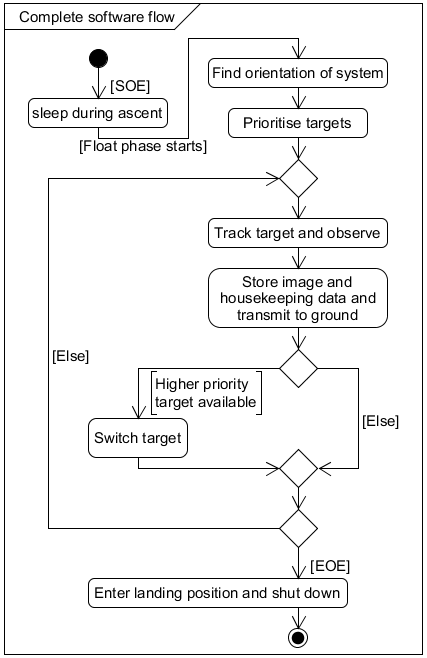
\includegraphics[width=.5\textwidth]{4-experiment-design/img/software/activity-diagram.png}
    \caption{Activity diagram describing the complete software flow. Here the internal actions SOE and EOE refer to when the software starts, i.e. on the launch pad, and shuts down respectively. This is done independently and therefore requires no activity from the gondola.}
    \label{fig:software-activity-diagram}
\end{figure}

\begin{figure}[H]
    \centering
    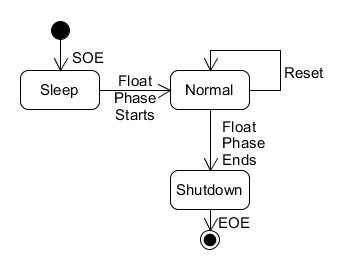
\includegraphics[width=.7\textwidth]{4-experiment-design/img/software/state-diagram.png}
    \caption{State diagram for On-Board Software.}
    \label{fig:software-state-diagram}
\end{figure}

\clearpage
\paragraph{f)} Modularisation and pseudo code

\begin{figure}[H]
    \centering
    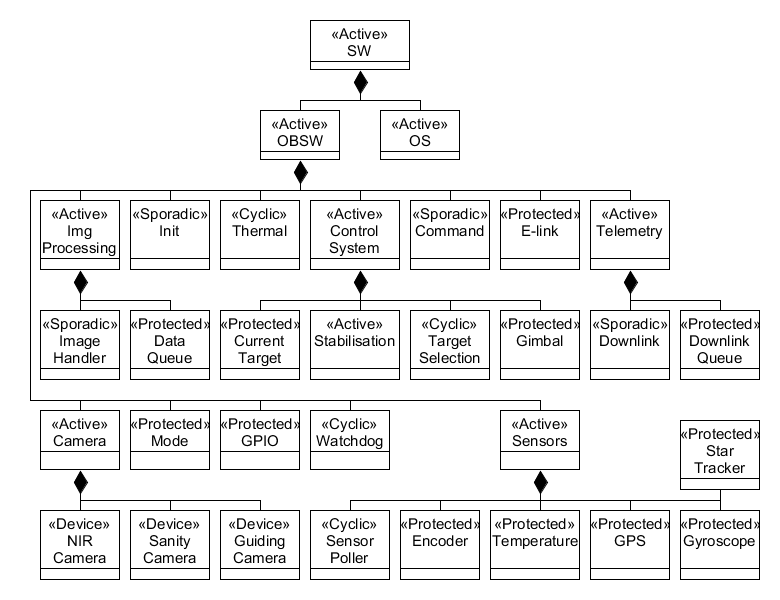
\includegraphics[width=\textwidth]{4-experiment-design/img/software/composition-tree.png}
    \caption{Composition tree of On-Board Software.}
    \label{fig:software-composition-tree}
\end{figure}

Figure \ref{fig:software-composition-tree} shows how the complete software was modularised. Each component is described below.

\begin{itemize}

    \item Camera: Parent
        \begin{itemize}
            \item Guiding Camera: Communication link to the guiding camera.
            \item NIR Camera: Communication link to the NIR camera.
        \end{itemize}

    \item Command: Module responsible for handling incoming commands from ground.

    \item E-link: Module responsible for communications over the E-link interface.

    \item GPIO: Module responsible for communications through the Raspberry Pi GPIO.

    \item Img Processing: Image processing, parent
        \begin{itemize}
            \item Data Queue: Buffer to hold camera data until Handler is ready
            \item Image Handler: Module processing and storing images taken by camera.
        \end{itemize}

    \item Init: Module initialising each component.

    \item Mode: Module responsible for the current state of the software.

    \item Sensors: Parent
        \begin{itemize}
            \item Encoder: Module holding encoder data.
            \item GPS: Module holding GPS data.
            \item Gyroscope: Module holding gyroscope data.
             \item Sensor Poller: Module responsible for polling sensors.
            \item Star Tracker: Module holding absolute attitude obtained from the star tracker.
            \item Temperature: Thermal sensors.
        \end{itemize}

    \item Telemetry: Parent
        \begin{itemize}
            \item Downlink: Module responsible for sending telemetry to ground.
            \item Downlink Queue: Buffer to hold telemetry messages.
        \end{itemize}

    \item Thermal: Module responsible for active thermal control

    \item Control System: Parent
        \begin{itemize}
            \item Current Target: Module holding the current target to be observed.
            \item Controller: Module responsible for keeping camera on target.
            \item Gimbal: Module providing an interface to the gimbal motors.
            \item Target Selection: Module responsible for keeping track of target prioritisation and positioning as well as controlling the main camera.
        \end{itemize}

    \item Watchdog: Timer to reset watchdog.

\end{itemize}

\subsubsection{Implementation}

The code for the On-Board Software was implemented in C. An operating system was used to enable the modularisation required. The chosen operating system was Arch Linux ARM. Additional libraries used were: the ASI SDK library for controlling the cameras, zstd for data compression, cfitsio for handling .fit files, and ftd2xx for communications with the gyroscope.

\subsubsection{Unit Tests Performed}

\paragraph{Cameras}

The same software was used for the two ZWO cameras and therefore only the NIR camera was used in the test since it has the highest resolution and therefore higher requirements in terms of computer resources. The OBSW was compared against software provided by ZWO to see that it works as expected. A test was also performed to compare noise levels from the camera while using the USB 2.0 and 3.0 interfasces. The methodology and results are presented in Appendix \ref{app:camera_software_test}.

\paragraph{GPS receiver}

The GPS receiver and the OBSW controlling it was tested on a road trip across Sweden. The horizontal positioning was evaluated using Google satellite imaging and the altitude is evaluated using SRTM1 data to verify adequate accuracy. The methodology and results are presented in Appendix \ref{app:gps_test}. The GPS data from the receiver was deemed to be accurate.


\subsubsection{Control system}
The main task of the control system was selecting and tracking the astronomical targets and stabilising the telescope during exposure. Other tasks included minor tasks like the thermal control of the CMOS sensor and the electronics box as well as control of the actuators. A general overview of the control loop for tracking \& stabilisation is given in figure  \mbox{\ref{fig::software::control_loop}} below. The thermal control loop is sketched in chapter \mbox{\ref{Thermal_section}}.

\paragraph{Selecting and tracking targets}

The selection and tracking of targets was done by using the current time, position (GPS) and orientation star tracker and gyroscope) of the gondola. Once a suitable target in the operational field of view was selected, it was tracked during exposure. This included the compensation of the following motions:
\begin{itemize}
    \item Time-dependent rotational motion of the astronomical targets in the sky. This will be continuously compensated during exposure using models and/or interpolation of tables.
    \item Position-dependent rotational motion of the astronomical targets in the sky. This will be corrected once for every picture, using the GPS data.
    \item Rotation of the gondola in the z-axis; can be corrected during exposure using a gyroscope sensor.
\end{itemize}

Due to the nature of the motion of astronomical targets, it is necessary to use a 3-axis gimbal.

\paragraph{Selection of targets}

The selection of targets was based on the operational field of view (the area of the sky where the telescope is able to look at) and prioritisation parameters of the possible targets within this field of view. The operational field of view was determined by using the sensor data from the orientation sensor (star tracker). Using a star tracker provided an accurate absolute attitude determination system to ensure that the celestial object of interest was actually in the field of view of the telescope when it was pointed there. Compared to the gyroscopes that have a much higher angular resolution, the attitude determination system does not show any drift over time and does therefore not need to be calibrated during flight.

Prioritisation parameters included the brightness of the object (brighter objects are expected to yield better results due to higher SNR), the location of the object within the operational field of view (objects near the centre of the field of view are favoured because they are less likely to rotate out of the field of view during exposure) and the number of exposures already taken (objects should be imaged more than once in order to be able to compare and verify the obtained data, but not more often than ten times during the flight). 

As the location of the astronomical targets changes with time and position of the gondola, these two parameters also need to be taken into account (for determination see paragraph Astronomical targets). Once a target was selected, this part of the control system was deactivated until the picture was taken or the control loop was re-initialised.

The 4 chosen prioritisation parameters were:
\begin{itemize}
    \item No. of exposures already taken (exposure parameter)
    \item Magnitude of the target (constant)
    \item Position parameter
    \item Type of target  (defined scientific parameter, constant)
\end{itemize}

The exposure parameter depends on the number of images of the target that have already been taken, and was defined as follows: \texttt{exp\_param\_list = [1,2,3,4,4,4,3,2,1,1,1]} for 0 to 9 exposures respectively, and 0 for all other. This ensured that not more than 10 images are taken (maximum defined in the scientific requirements) and that targets with more than 2 exposures were prioritised in order to get sufficient scientific data of one target.

The magnitude of the target is defined by the target itself and is therefore constant. Typical values range from 3 to 10 for the chosen targets. The higher the value the brighter the target, and therefore more suitable to observe.

The position parameter depends on the gondola attitude and was recalculated based on the current time, position and attitude each time. It was then calculated as follows: if the absolute difference between the gondola attitude and the target position is smaller than a set value (e.\,g.~maximum telescope range - $\ang{30}$) it was defined as 
\begin{align*}
    \left|\text{gondola attitude} - \text{target position} \right|
\end{align*}
otherwise as zero. This means that no targets that are outside the field of view were chosen, and the most central targets were preferred in order to minimise the risk of the target rotating out of the field of view during exposure.

The type of target (nebula/galaxy/open cluster/globular cluster) prioritises nebulae and galaxies to cluster. The prioritisation order was \texttt{type\_param\_list = [4,3,2,1]} for the order mentioned above.

To get a final prioritisation value for each target, all prioritisation parameters were multiplied. This ensured that targets outside the field of view as well as targets with 10 exposures were not taken into consideration any more, as the result is 0. The target with the highest calculated prioritisation value was selected for the next exposure.



\paragraph{Tracking of astronomical targets}

The time-dependent and the position-dependent rotational motion of the astronomical targets was calculated by using an astronomical model and provided the control input for the subsequent stages of the control system. Because the state vectors for this model are time (internal clock) and position (GPS) and the input vector is the selected target (defined in the system, not a variable state for the exposure of one image), the state vectors cannot be affected by the control system (not controllable). Therefore, no dedicated feedback loop was used for this part of the control system. The output vector then provided the input for the compensation of rotation (of the gondola in the z-axis) and the stabilisation of the gimbal.

The astronomical model used to determine the current position of the targets was the Alt Az (Altitude Azimuth) reference frame. It defines the position of the astronomical target with respect to geographic north and zenith and depends on current the time, date and position of the observer. It is calculated based on the RA DEC (Right Ascension, Declination) of the astronomical target. The formulas required for this conversion are given in \mbox{\cite{RaDec2AltAz}}.

Figure \mbox{\ref{fig::software::position_map}} shows the positions of the IRISC targets on October 31st, 12:00, 2019 in Esrange as simulated by the tracking algorithm in MATLAB. The positions are accurate within arcminutes if compared with commercial astronomy software for the absolute position. The difference that occurs within one $\SI{30}{\s}$ exposure is negligible. The same would be true for exposures of several hours.

To illustrate the necessity of tracking figure \mbox{\ref{fig::software::star_trails}} shows a simulated exposure of 5h of all IRISC targets starting on October 31, 12:00, 2019 in Esrange (with the position held constant). 

\begin{figure}[htb]
    \centering
    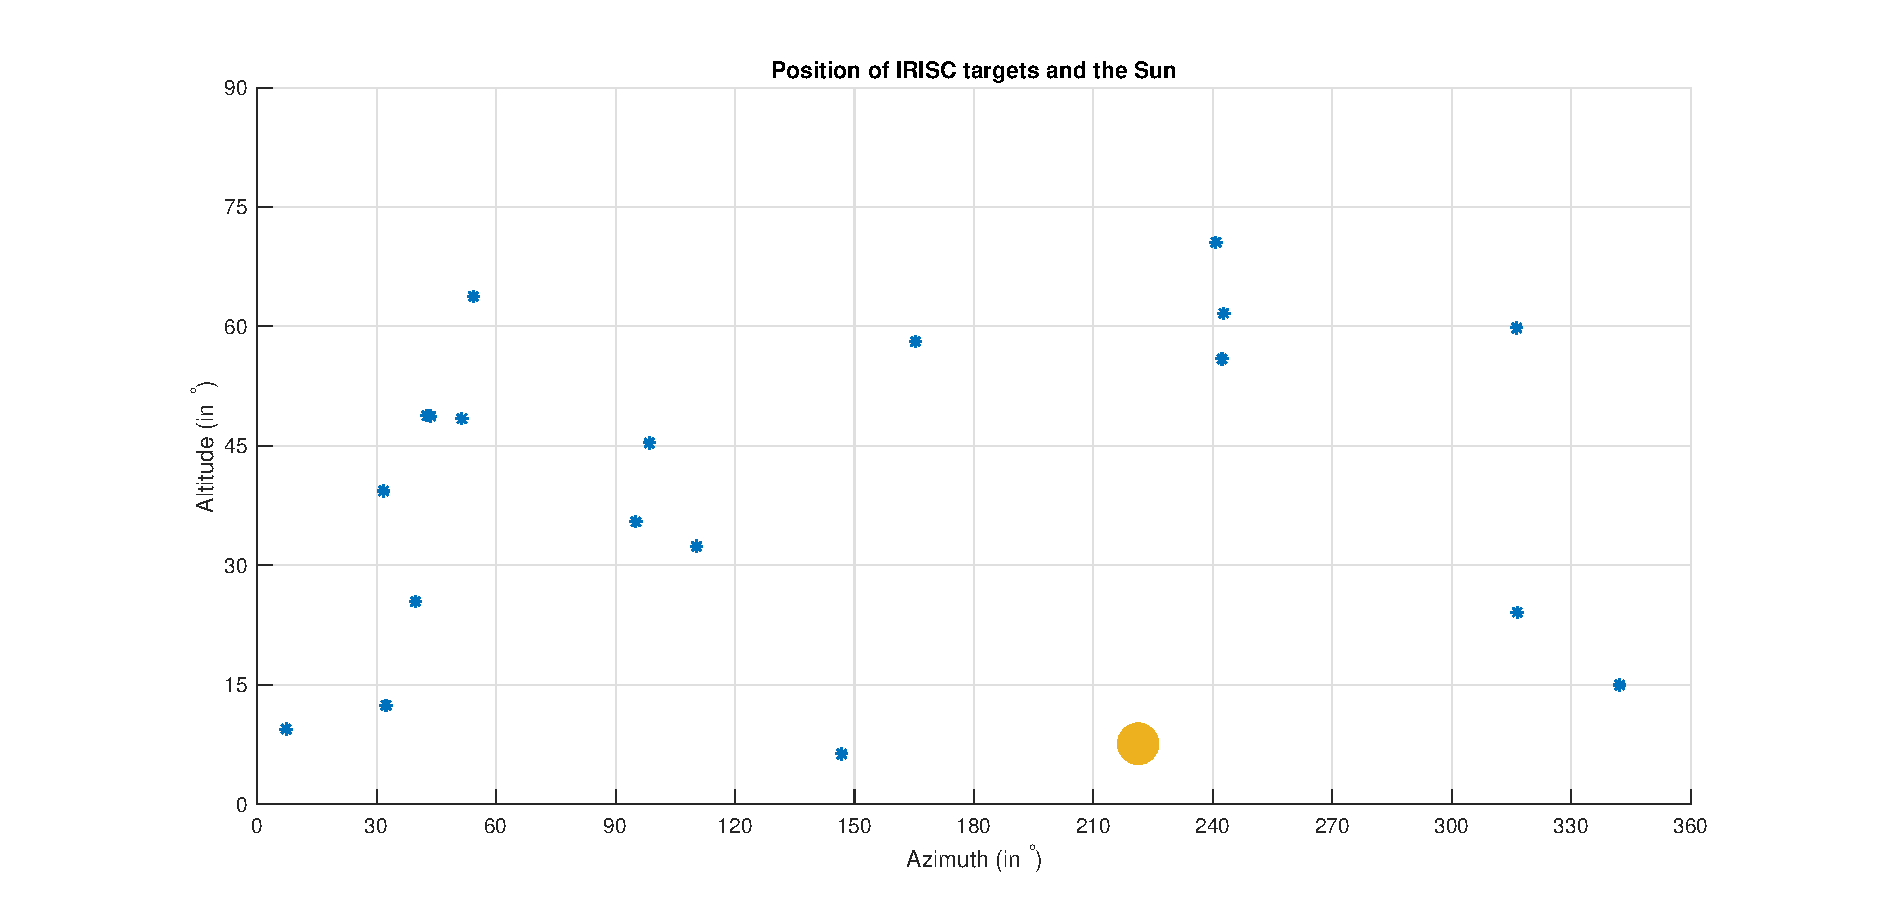
\includegraphics[width = \textwidth]{4-experiment-design/img/software/position_map_31-10-19_12-00.eps}
    \caption{MATLAB simulation of the tracking algorithm showing all visible IRISC targets and the Sun on October 31, 12:00, 2019 in Esrange}
    \label{fig::software::position_map}
\end{figure}
\begin{figure}[htb]
    \centering
    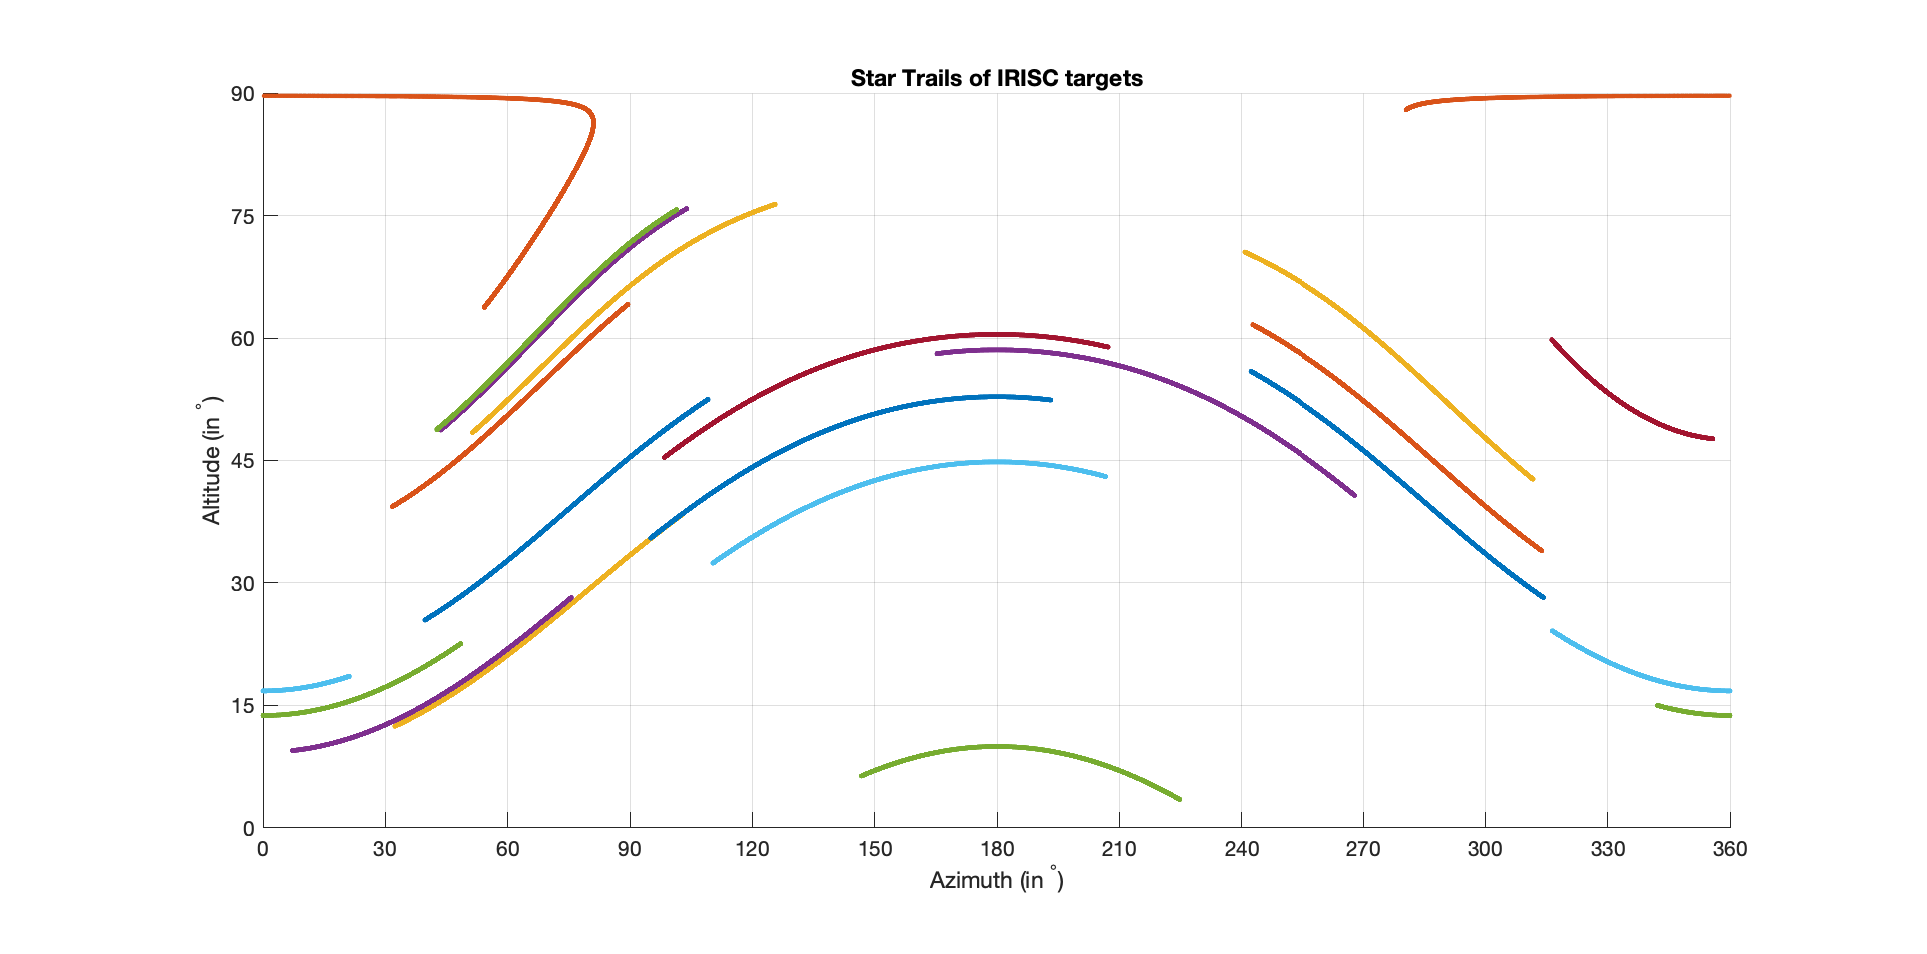
\includegraphics[width = \textwidth]{4-experiment-design/img/software/star_trails_31-10-19_12-00.eps}
    \caption{MATLAB simulation of the tracking algorithm showing all visible IRISC targets and the Sun on October 31, 12:00, 2019 in Esrange}
    \label{fig::software::star_trails}
\end{figure}

\paragraph{Rotation of the gondola}

The uncontrolled rotational motion of the gondola around the z-axis could be directly compensated by actuating the corresponding gimbal axis (yaw). This was achieved by a PID control. As the same axis was also actuated during the stabilisation process, it was merged with the control loop for the stabilisation. As the required accuracy for detecting the rotation of the gondola was very high, the gyroscopes were used to provide the input (see stabilisation for more detail).



\paragraph{Stabilisation of the gimbal}

The stabilisation of the gimbal only needed to be active during exposure in order to avoid blurred pictures. However, to simplify implementation and improve the performance of the star tracker it was enabled the entire time once the system went into the mode responsible for taking images. It was responsible for compensating all kinds of small-scale, unpredicted movements of the gondola. In order to achieve this, an active feedback loop that requires information about the gondola movements was needed. The sensor data for the feedback loop was provided by the Kalman filter using the gyroscope and the star tracker. This setup has the accuracy (angular resolution) of the gyroscope while also being bias-compensated and providing not only the relative motion of the telescope but also the absolute pointing within the accuracy of the star tracker.

In addition to the gyroscopes, the encoders were used to obtain the actual position of the telescope within the gondola. The sensor data was filtered by a Kalman filter to decrease the sensor noise and deduce the current orientation of the telescope as well as the motion of the gondola with a high precision.

The control of the gimbal (tracking and stabilisation as well as compensation of the gondola rotation for the yaw axis) was done by a separate PID control for each axis. The output of the controller was the required speed for the actuating motor of the respective axis. This information was then processed by the motor controller that calculated the required input for the motors.

The stabilisation algorithm was written in C as most of the OBSW. The team refrained from using third party libraries, so the whole stabilisation code is built using standard C libraries. The analysis was conducted on a Simulink model and acquired PID values were tested on the instrument during integration tests.

\paragraph{Attitude determination - Kalman filter}

The Kalman filter utilised the measured data from the gyroscope to predict the current angle of the telescope and fused this predicted value with the absolute orientation of the telescope obtained by the star tracker in the update step of the Kalman filter. As the gyroscope only measures angular rates the absolute orientation cannot be determined without a reference value. Also, sensor noise and imperfections, e.\,g.~gyro bias result in a drift of the predicted values. As the gyroscope was sampled with a much higher frequency than the star tracker due to the necessary exposure time of the star tracker camera as well as the calculation time of the star tracker on the onboard software, the update step (sensor fusion of gyroscope data and star tracker data) was only done when a new set of data from the star tracker was available, while the prediction step using only the gyroscope data was done with the same sampling time as the gyroscope readout. 
Additionally, the computation time of the star tracker was higher than the exposure time of the guiding camera and was therefore not negligible because the obtained results are outdated, resulting in wrong prediction of the bias drift and subsequently also the position of the telescope. To compensate this a subset of the most recent gyroscope measurements and position estimates was temporarily stored during the prediction of the Kalman filter when no new star tracker data was available. For the update step the Kalman filter went back in time and took the position estimates from the time when the star tracker result was valid (i.\,e.end of exposure). It used these estimates along with the stored gyroscope data to conduct the update step and re-predict the current position estimates of the telescope.
 The development including testing of this algorithm was done in MATLAB, while for the OBSW it was written in c. A simulation of the performance of the Kalman filter can be seen in figure \mbox{\ref{fig::software::Kalman_filter}} to \mbox{\ref{fig::software::Kalman_filter_delay_2}}. 
The sampling frequency of the gyroscope is $\SI{40}{\Hz}$ while the star tracker is sampled at $\SI{30}{\second}$ for figure \mbox{\ref{fig::software::Kalman_filter}}. The blue lines show the actual error of the values estimated by the Kalman filter, while the black lines demonstrate a standard deviation of 1 ($\SI{68}{\percent}$) of an optimally tuned Kalman filter. 
Figure \mbox{\ref{fig::software::Kalman_filter}} shows the error of the position and bias estimates for the Kalman filter with a gyroscope sampling frequency of $\SI{40}{\Hz}$ and a star tracker sampling time of $\SI{30}{\second}$ but no additional star tracker delay. Figure \mbox{\ref{fig::software::Kalman_filter_delay_1}} shows the Kalman filter with a gyroscope sampling frequency of $\SI{40}{\Hz}$ and a star tracker sampling time of $\SI{10}{\second}$ with a delay of $\SI{8}{\s}$ and a linear angular speed profile of $\SI{1}{\degree\per\s}$ which was the upper estimated limit of the gondola rotation. Figure \mbox{\ref{fig::software::Kalman_filter_delay_2}} has a periodically oscillating angular rotation profile with the period time corresponding to an ideal pendulum with a length of $\SI{100}{\m}$ and a maximum displacement of approx. $\ang{1}$ (half angle). This simulated the expected swinging motion of the gondola. All three scenarios showed that the Kalman filter can handle the different sampling rates and delay times of the star tracker as well as the expected angular speed profiles of the balloon. The oscillating motion in figure \mbox{\ref{fig::software::Kalman_filter_delay_2}} gets stronger with a higher maximum angular offset and nearly disappears for dislocations below $\ang{0.5}$ (half angle).

\begin{figure}[htb]
    \centering
    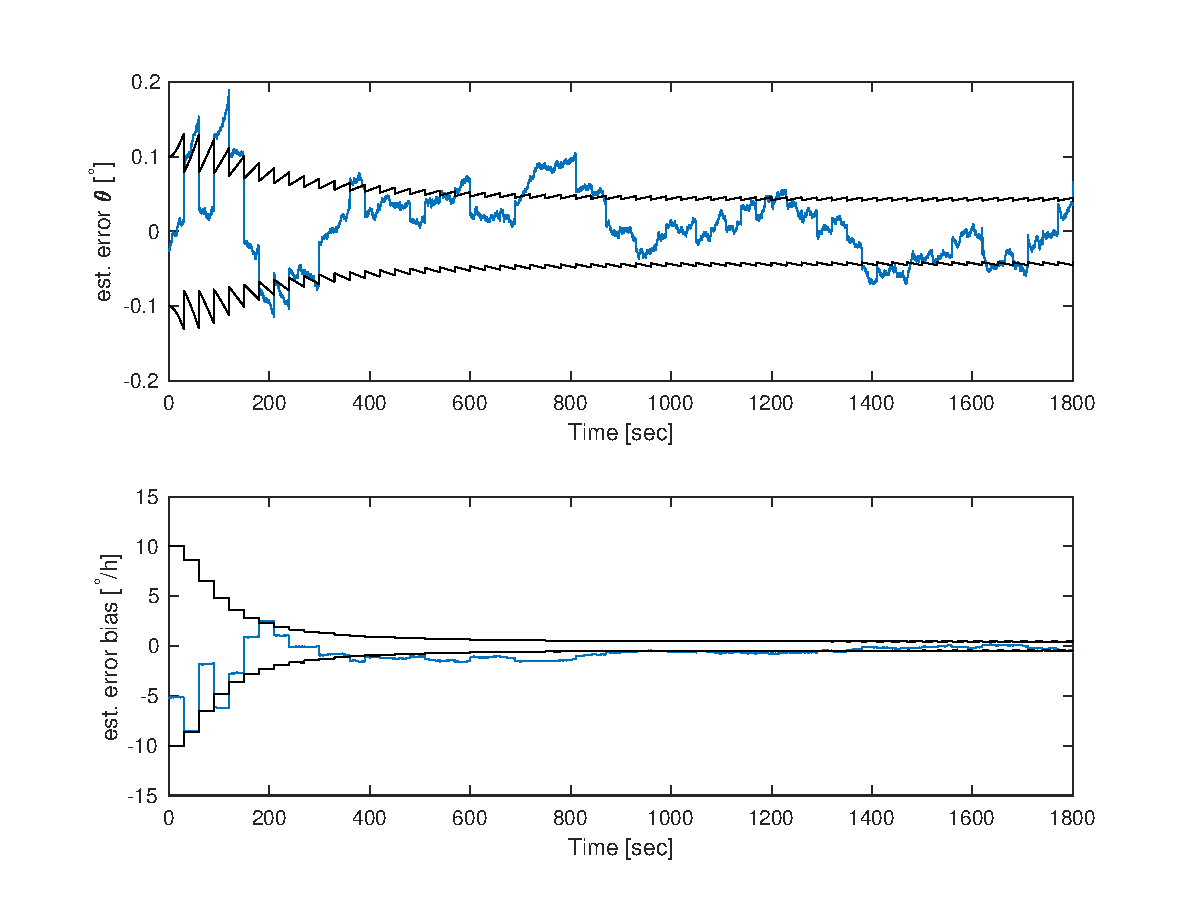
\includegraphics[width = 0.8\textwidth]{4-experiment-design/img/software/kf_30_0_lin.eps}
    \caption{MATLAB simulation of the Kalman filter with noise distribution of the gyroscope according to the data sheet}
    \label{fig::software::Kalman_filter}
\end{figure}
\begin{figure}[htb]
    \centering
    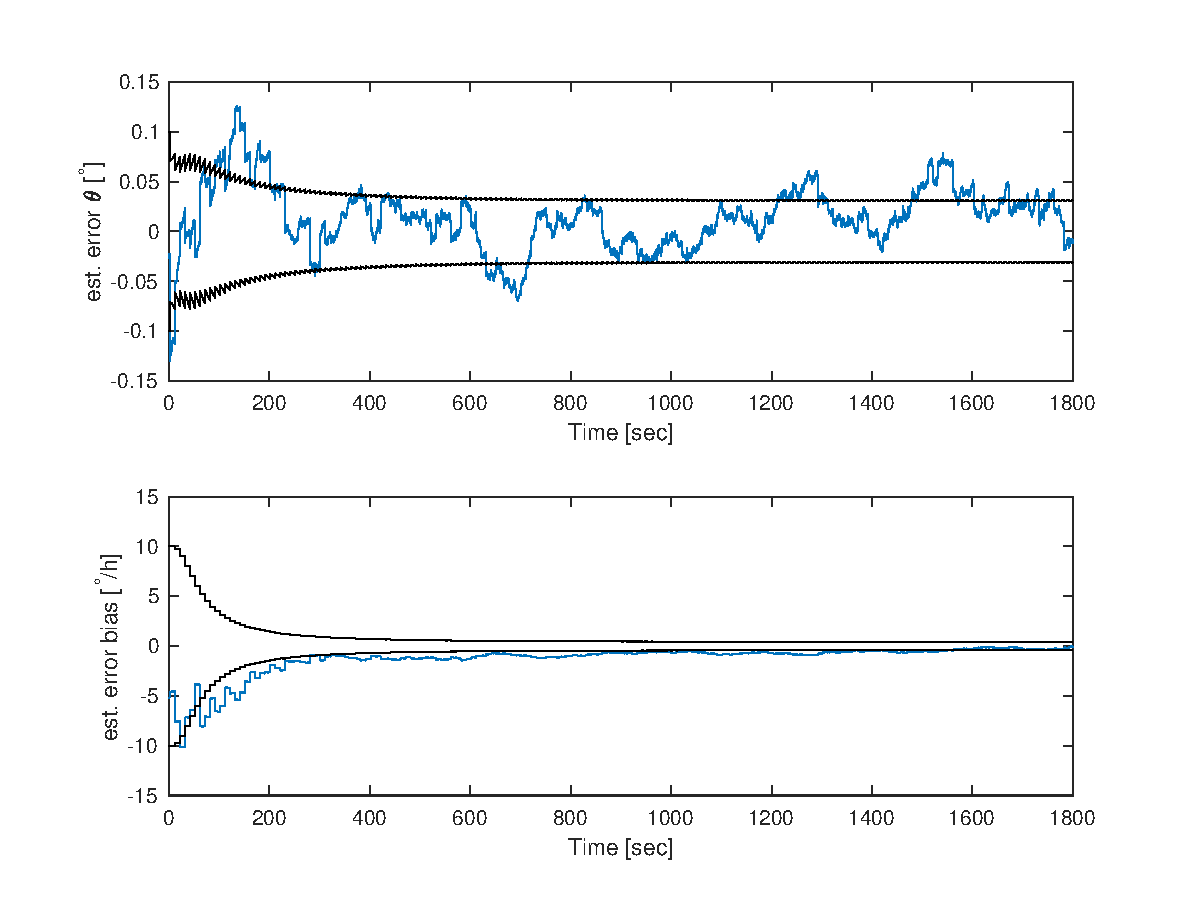
\includegraphics[width = 0.8\textwidth]{4-experiment-design/img/software/kf_10_8_lin.eps}
    \caption{MATLAB simulation of the Kalman filter including star tracker delay for a linear angular rotation profile}
    \label{fig::software::Kalman_filter_delay_1}
\end{figure}
\begin{figure}[htb]
    \centering
    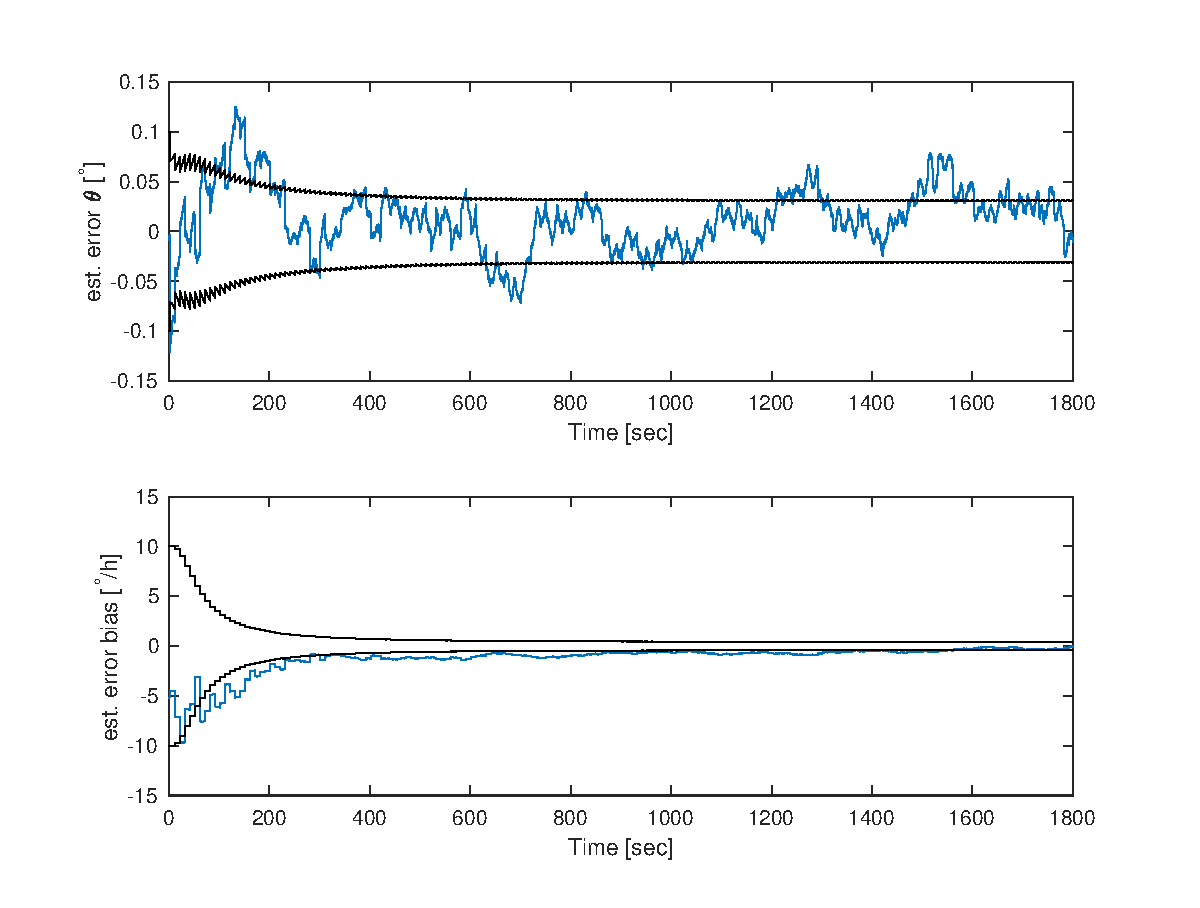
\includegraphics[width = 0.8\textwidth]{4-experiment-design/img/software/kf_10_8_cos_3_1800.eps}
    \caption{MATLAB simulation of the Kalman filter including star tracker delay for a periodic angular rotation profile}
    \label{fig::software::Kalman_filter_delay_2}
\end{figure}

\newpage
\begin{landscape}
    \begin{figure}
        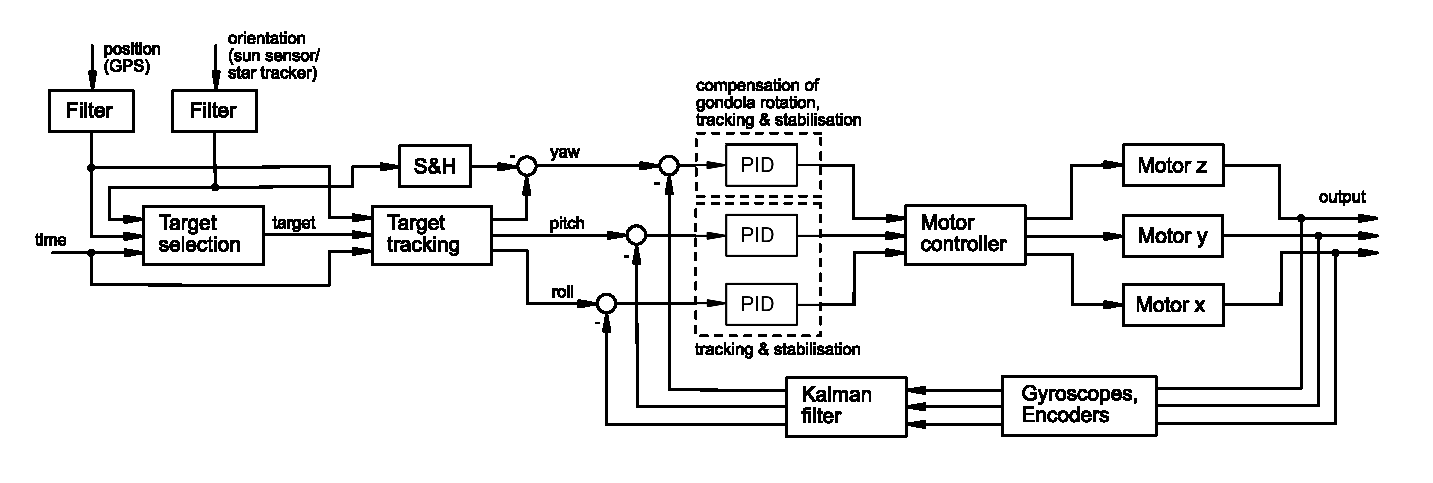
\includegraphics[width=\linewidth]{4-experiment-design/img/software/Control_loop.eps}
        \caption{Control loop of the experiment}
        \label{fig::software::control_loop}
    \end{figure}
\end{landscape}


\raggedbottom
